%----------------------------------------------------------------------------------------
%	PACKAGES AND THEMES
%----------------------------------------------------------------------------------------
\documentclass[aspectratio=169,xcolor=dvipsnames]{beamer}
\usetheme{Madrid}
% \usepackage[backend=bibtex, defernumbers=true, style=numeric, citestyle=ieee]{biblatex}
% \addbibresource{ref.bib}
\usepackage{hyperref}
\graphicspath{{./images/}}
\usepackage{graphicx} % Allows including images
\usepackage{booktabs} % Allows the use of \toprule, \midrule and \bottomrule in tables
\usepackage[utf8]{inputenc}
\usepackage[T1]{fontenc}
\usepackage{amsmath,amssymb}
\usepackage{multirow}
\usepackage{array}
\usepackage{tikz}
\usetikzlibrary{positioning}

%----------------------------------------------------------------------------------------
%	TITLE PAGE
%----------------------------------------------------------------------------------------

% The title
\title[Project Crypto Java]
{
	Plateforme de Cryptographie Sécurisée
}

\subtitle{Soutenance de Projet - Master TDSI}
\author[MTDSI]{Étudiant(e)s \and Professeur : Pr. Demba SOW}

\date{\today} 


%----------------------------------------------------------------------------------------
%	PRESENTATION SLIDES
%----------------------------------------------------------------------------------------

\begin{document}

\begin{frame}
    % Print the title page as the first slide
    \titlepage
\end{frame}

\begin{frame}{Plan de la présentation}
    \tableofcontents
\end{frame}

%------------------------------------------------

\section{Introduction et Objectifs}
\begin{frame}{Contexte et Objectifs}
	Le projet vise à fournir une plateforme web complète et sécurisée permettant de réaliser diverses opérations cryptographiques :\\
	\vspace{0.03\textheight} 
	\begin{itemize}
		\item Chiffrement et déchiffrement de fichiers.
		\item Hachage et vérification d'intégrité.
		\item Signature numérique et validation.
		\item Gestion sécurisée des clés asymétriques et symétriques.
	\end{itemize}
	\vspace{0.03\textheight}
	Une attention particulière a été portée sur l'architecture robuste, la sécurité des accès, et la supervision du système.
\end{frame}

%------------------------------------------------

\section{Architecture Globale}
\begin{frame}{Architecture de la Plateforme}
	L'application repose sur une architecture moderne à trois niveaux :
	
	\begin{block}{Frontend (React.js \& Nginx)}
		Interface utilisateur interactive et ergonomique, construite en React et distribuée par un serveur web Nginx (faisant office de reverse proxy).
	\end{block}
	
	\begin{alertblock}{Backend (Java Spring Boot)}
		API REST robuste gérant la logique métier, les opérations cryptographiques et la sécurité (Spring Security).
	\end{alertblock}
	
	\begin{examples}{Base de Données (MySQL 8.0)}
		Persistance relationnelle sécurisée des utilisateurs, des clés publiques, et des journaux d'audit (Audit Logs).
	\end{examples}
\end{frame}

%------------------------------------------------

\section{Modèle de Données}
\begin{frame}{Schéma Relationnel de la Base de Données}
	\begin{center}
	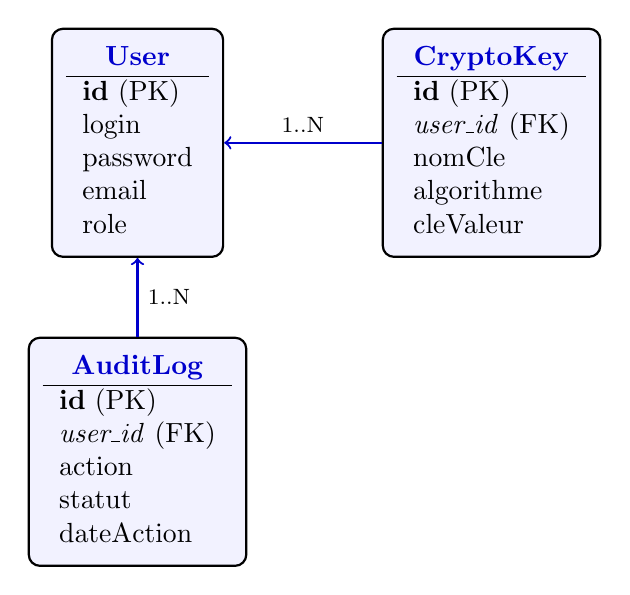
\begin{tikzpicture}[
	  table/.style={draw, thick, rounded corners, fill=blue!5, inner sep=5pt},
	]
	
	% Table User
	\node[table] (user) {
		\begin{tabular}{l}
			\multicolumn{1}{c}{\textcolor{blue!80!black}{\textbf{User}}} \\
			\hline
			\textbf{id} (PK) \\
			login \\
			password \\
			email \\
			role \\
		\end{tabular}
	};
	
	% Table CryptoKey
	\node[table, right=2cm of user] (key) {
		\begin{tabular}{l}
			\multicolumn{1}{c}{\textcolor{blue!80!black}{\textbf{CryptoKey}}} \\
			\hline
			\textbf{id} (PK) \\
			\textit{user\_id} (FK) \\
			nomCle \\
			algorithme \\
			cleValeur \\
		\end{tabular}
	};
	
	% Table AuditLog
	\node[table, below=1cm of user] (log) {
		\begin{tabular}{l}
			\multicolumn{1}{c}{\textcolor{blue!80!black}{\textbf{AuditLog}}} \\
			\hline
			\textbf{id} (PK) \\
			\textit{user\_id} (FK) \\
			action \\
			statut \\
			dateAction \\
		\end{tabular}
	};
	
	% Relations (Arrows)
	\draw[<-, thick, draw=blue!80!black] (user.east) -- node[above, font=\footnotesize] {1..N} (key.west);
	\draw[<-, thick, draw=blue!80!black] (user.south) -- node[right, font=\footnotesize] {1..N} (log.north);
	
	\end{tikzpicture}
	\end{center}
\end{frame}

\begin{frame}{Preuve : Base de Données (MySQL)}
	\begin{figure}
		\centering
		% Remplacer "example-image" par le nom de votre capture d'écran (ex: capture-bdd.png)
		\includegraphics[width=0.8\linewidth, height=0.6\textheight, keepaspectratio]{example-image}
		\caption{Capture d'écran : Tables et données (ex: phpMyAdmin ou console MySQL)}
	\end{figure}
\end{frame}

%------------------------------------------------

\section{Sécurité Applicative (Spring Security \& JWT)}

\begin{frame}{Sécurisation de l'API avec Spring Security}
	L'application protège ses ressources de manière rigoureuse en utilisant \textbf{Spring Security} :
	\vspace{0.03\textheight}
	\begin{itemize}
		\item \textbf{Filtres d'Interception (FilterChain)} : Toute requête HTTP entrante est interceptée et analysée avant d'atteindre la logique métier.
		\item \textbf{AuthenticationManager} : Responsable de valider les identifiants (mot de passe haché) lors de la tentative de connexion via l'interface \texttt{UserDetailsService}.
		\item \textbf{Protection des Endpoints} : Verrouillage strict de l'API REST. Seul l'endpoint de connexion (\texttt{/auth/login}) est public ; tous les autres exigent une authentification valide.
	\end{itemize}
\end{frame}

\begin{frame}{Authentification Stateless : JSON Web Token (JWT)}
	Pour gérer les sessions sans surcharger la mémoire du serveur (\textit{Stateless}), l'application s'appuie sur la norme \textbf{JWT}.
	\vspace{0.03\textheight}
	\begin{block}{Génération et Utilisation du Jeton}
		\begin{enumerate}
			\item \textbf{Création} : Lors d'un login réussi, le backend génère un jeton contenant les informations de l'utilisateur (Payload).
			\item \textbf{Signature Cryptographique} : Ce jeton est \textbf{signé numériquement} (souvent avec un HMAC-SHA256) pour garantir qu'il ne soit jamais falsifié par le client.
			\item \textbf{Transmission} : Le client stocke le jeton et l'envoie dans l'en-tête HTTP (\texttt{Authorization: Bearer <token>}) à chaque nouvelle requête. Le filtre Spring vérifie alors la signature avant d'autoriser l'accès.
		\end{enumerate}
	\end{block}
\end{frame}

\begin{frame}{Implémentation : Le Package \texttt{config}}
	L'architecture de sécurité est centralisée dans le package \textbf{\texttt{config}}, qui orchestre ces mécanismes via plusieurs classes dédiées :
	\vspace{0.02\textheight}
	\begin{itemize}
		\item \textbf{\texttt{SecurityConfig}} : Cœur de la sécurité. Définit la \texttt{SecurityFilterChain}, désactive le CSRF (inutile en Stateless), et configure les autorisations d'URL.
		\item \textbf{\texttt{JwtAuthenticationFilter}} : Composant critique (\texttt{OncePerRequestFilter}) interceptant chaque requête HTTP pour extraire, vérifier et valider la signature du jeton JWT.
		\item \textbf{\texttt{JwtUtils}} : Utilitaire cryptographique gérant la création du jeton, sa signature HMAC-SHA, et l'extraction sécurisée des données (Claims).
		\item \textbf{\texttt{ApplicationConfig} \& \texttt{CorsConfig}} : Injection de l'\texttt{AuthenticationProvider}, du \texttt{PasswordEncoder} (BCrypt), et gestion des requêtes cross-origin pour React.
	\end{itemize}
\end{frame}

\begin{frame}{Preuve : Authentification et JWT}
	\begin{figure}
		\centering
		% Remplacer "example-image" par le nom de votre capture d'écran (ex: capture-jwt.png)
		\includegraphics[width=0.8\linewidth, height=0.6\textheight, keepaspectratio]{example-image}
		\caption{Capture d'écran : Obtention du jeton (Postman/Swagger) et accès sécurisé}
	\end{figure}
\end{frame}

%------------------------------------------------

\section{Cryptographie (JCA \& JCE)}

\begin{frame}{Architecture Cryptographique Java (JCA/JCE)}
	\begin{block}{Cryptographic Service Provider (CSP)}
		Le moteur de sécurité de l'application repose sur l'architecture standard de Java (\textbf{JCA} et \textbf{JCE}).
		\begin{itemize}
			\item \textbf{Provider natif} : Java propose par défaut des fournisseurs comme \texttt{SunJCE} et \texttt{SunRsaSign}.
			\item \textbf{Provider tiers (Bouncy Castle)} : Pour pallier certaines limitations (comme les restrictions de tailles de clés) et intégrer des algorithmes modernes, le \textbf{\texttt{BouncyCastleProvider}} a été enregistré dynamiquement via la classe \texttt{Security} au démarrage du Backend.
		\end{itemize}
	\end{block}
\end{frame}

\begin{frame}{Gestion des Clés}
	\begin{alertblock}{Clés Symétriques (\texttt{javax.crypto.SecretKey})}
		Générées via la classe d'engine \textbf{\texttt{KeyGenerator}} \\
        Exemple : \texttt{KeyGenerator.getInstance("AES", "BC")} \\
		Elles garantissent une très haute performance pour le chiffrement de fichiers volumineux.
	\end{alertblock}
	
	\begin{examples}{Paires de Clés Asymétriques (\texttt{java.security.KeyPair})}
		Générées via \textbf{\texttt{KeyPairGenerator}} \\
        Exemple : \texttt{KeyPairGenerator.getInstance("RSA", "BC")} \\
		Les interfaces \texttt{PublicKey} et \texttt{PrivateKey} sont utilisées pour l'authentification et l'échange sécurisé.
	\end{examples}
\end{frame}

\begin{frame}{Gestion des Clés : Persistance et Sérialisation}
	Afin de pouvoir réutiliser une clé secrète générée, l'application implémente des mécanismes de persistance physique via la \textbf{Sérialisation Java}.
	\vspace{0.02\textheight}
	\begin{itemize}
		\item \textbf{Sauvegarde (Export)} : Écriture de l'objet clé sur le disque physique à l'aide de \texttt{ObjectOutputStream.writeObject(secretKey)}.
		\item \textbf{Restauration (Import)} : Reconstruction de la clé en mémoire depuis le fichier de sauvegarde via \texttt{ObjectInputStream.readObject()}.
		\item \textbf{Vérification d'intégrité} : La comparaison des objets (\texttt{sk.equals(sk2)}) confirme que la clé chargée est mathématiquement identique à la clé générée, sans aucune altération.
	\end{itemize}
\end{frame}

\begin{frame}{Processus de Chiffrement et Déchiffrement}
	\begin{block}{Cryptographie Symétrique (ex: AES)}
		\textbf{Principe} : Une même clé secrète sert à chiffrer et déchiffrer. L'algorithme découpe les données en blocs (mode CBC) et utilise un Vecteur d'Initialisation (IV) pour garantir l'aléatoire.\\
		\textbf{Code} : \texttt{cipher.init(Cipher.ENCRYPT\_MODE, secretKey, ivSpec)} puis \texttt{doFinal()}
	\end{block}
	
	\begin{block}{Cryptographie Asymétrique (ex: RSA)}
		\textbf{Principe} : Utilisation d'un bi-clé. La \textbf{Clé Publique} chiffre le message (accessible à tous), mais seule la \textbf{Clé Privée} (gardée secrète) peut le déchiffrer. Ce processus est mathématiquement lourd mais idéal pour échanger des clés de session de manière sécurisée.\\
		\textbf{Code} : \texttt{cipher.init(Cipher.DECRYPT\_MODE, privateKey)}
	\end{block}
\end{frame}

\begin{frame}{Fonctions de Hachage et HMAC}
	\begin{alertblock}{Le Hachage (ex: SHA-256)}
		\textbf{Principe} : Fonction mathématique à sens unique (\textit{one-way}). Elle prend un document de taille variable et retourne une empreinte numérique unique de taille fixe. Une infime modification du document change totalement l'empreinte (\textit{effet avalanche}).\\
		\textbf{Code} : \texttt{MessageDigest.getInstance("SHA-256", "BC").digest(data)}
	\end{alertblock}
	
	\begin{examples}{Le HMAC (Hashed Message Authentication Code)}
		\textbf{Principe} : C'est un hachage combiné à une \textbf{Clé Secrète}. Il garantit à la fois que le fichier n'a pas été altéré (intégrité) ET qu'il provient bien d'une source autorisée (authentification).\\
		\textbf{Code} : \texttt{Mac.getInstance("HmacSHA256", "BC").doFinal(data)}
	\end{examples}
\end{frame}

\begin{frame}{Le Mécanisme de la Signature Numérique}
	La signature numérique garantit de façon asymétrique l'origine (\textbf{Authentification}) et l'impossibilité de nier l'envoi (\textbf{Non-Répudiation}).
	\vspace{0.03\textheight}
	\begin{itemize}
		\item \textbf{1. Émission (Signature)} : L'expéditeur hache d'abord le document pour obtenir son empreinte. Il \textbf{chiffre ensuite cette empreinte avec sa Clé Privée} (\texttt{signature.initSign(privateKey)} puis \texttt{sign()}).
		\item \textbf{2. Réception (Vérification)} : Le destinataire utilise la \textbf{Clé Publique} de l'expéditeur pour déchiffrer la signature (\texttt{signature.initVerify(publicKey)}).
		\item \textbf{3. Validation} : Si l'empreinte déchiffrée (\texttt{verify()}) correspond exactement au hachage local du document, ce dernier est 100\% authentique et intact.
	\end{itemize}
\end{frame}

\begin{frame}{Preuve : Opérations Cryptographiques}
	\begin{figure}
		\centering
		% Remplacer "example-image" par le nom de votre capture d'écran (ex: capture-crypto.png)
		\includegraphics[width=0.8\linewidth, height=0.6\textheight, keepaspectratio]{example-image}
		\caption{Capture d'écran : Chiffrement, hachage ou signature en cours d'exécution}
	\end{figure}
\end{frame}

%------------------------------------------------

\section{Infrastructure DevOps}
\begin{frame}{Conteneurisation : Docker \& Docker Compose}
	L'ensemble de l'application a été conteneurisé grâce à la technique du \textbf{Multi-Stage Build} pour optimiser le poids et la sécurité des images de production.
	
	\begin{table}
		\begin{tabular}{l l l}
			\toprule
			\textbf{Service Docker} & \textbf{Technologie} & \textbf{Rôle} \\
			\midrule
			\texttt{crypto\_frontend} & Nginx Alpine      & Serveur Web Statique Proxy \\
			\texttt{crypto\_backend}  & Eclipse Temurin 17& Serveur d'Application API \\
			\texttt{crypto\_mysql}    & MySQL 8.0         & Base de données \\
			\bottomrule
		\end{tabular}
		\caption{Orchestration via Docker Compose}
	\end{table}
\end{frame}

\begin{frame}{Orchestration : Kubernetes (K8s)}
	Pour garantir la haute disponibilité en production, le système a été traduit en manifestes Kubernetes :
	\vspace{0.03\textheight}
	
	\begin{itemize}
		\item \textbf{Deployments} : Gestion des instances (replicas) pour assurer la redondance du Backend et du Frontend.
		\item \textbf{Services} : Routage interne et exposition publique via \texttt{LoadBalancer}.
		\item \textbf{Secrets \& PVC} : Gestion sécurisée des mots de passe MySQL et persistance des données.
	\end{itemize}
\end{frame}

\begin{frame}{Preuve : Déploiement Docker \& Kubernetes}
	\begin{figure}
		\centering
		% Remplacer "example-image" par le nom de votre capture d'écran (ex: capture-docker.png)
		\includegraphics[width=0.8\linewidth, height=0.6\textheight, keepaspectratio]{example-image}
		\caption{Capture d'écran : Conteneurs actifs (\texttt{docker ps}) ou Pods Kubernetes}
	\end{figure}
\end{frame}

%------------------------------------------------

\section{Supervision (Monitoring)}
\begin{frame}{Supervision : Prometheus \& Grafana}
	\begin{block}{1. Collecte des Métriques (Actuator + Micrometer)}
		Le Backend Spring Boot expose en temps réel ses statistiques de santé : mémoire JVM, pics de CPU, utilisation des threads.
	\end{block}
	
	\begin{alertblock}{2. Prometheus}
		Une base de données temporelle qui "scrape" (aspire) ces données toutes les 15 secondes de manière autonome.
	\end{alertblock}

	\begin{examples}{3. Tableaux de Bord (Grafana)}
		Une interface graphique puissante interroge Prometheus pour afficher la charge serveur, le nombre de requêtes HTTP et configurer des alertes critiques.
	\end{examples}
\end{frame}

%------------------------------------------------

%------------------------------------------------

\section{Démonstration de l'Application}

\begin{frame}{Interface Utilisateur (Frontend React)}
	\begin{figure}
		\centering
		% Remplacer "example-image-a" par le chemin de votre image, ex: "images/frontend.png"
		\includegraphics[width=0.7\linewidth, height=0.5\textheight, keepaspectratio]{example-image-a}
		\caption{Espace de travail : Génération de clés et chiffrement}
	\end{figure}
\end{frame}

\begin{frame}{Documentation API (Swagger / OpenAPI)}
	\begin{figure}
		\centering
		% Remplacer "example-image-b" par le chemin de votre image, ex: "images/swagger.png"
		\includegraphics[width=0.7\linewidth, height=0.5\textheight, keepaspectratio]{example-image-b}
		\caption{Exploration et test des Endpoints de l'API REST}
	\end{figure}
\end{frame}

\begin{frame}{Supervision et Métriques (Grafana)}
	\begin{figure}
		\centering
		% Remplacer "example-image-c" par le chemin de votre image, ex: "images/grafana.png"
		\includegraphics[width=0.7\linewidth, height=0.5\textheight, keepaspectratio]{example-image-c}
		\caption{Tableau de bord : Surveillance de la charge et des ressources}
	\end{figure}
\end{frame}

%------------------------------------------------

\begin{frame}
    \Huge{\centerline{Merci de votre attention}}
    \vspace{0.05\textheight}
    \large{\centerline{Place aux questions et à la démonstration}}
\end{frame}

\end{document}
